% !TeX spellcheck = en-GB
\section{Materials \& Methods}
The automatic segmentation evolves around a Random Forest classifier. The whole segmentation pipeline is shown in \autoref{fig:pipeline}. The individual parts of the segmentation are covered in the following subsection. Furthermore the validation of the automatic segmentation is described.

To train the RF and evaluate the performance of the segmentation two data sets are used. The first data set comprises twenty MRI volumes and their ground truth. This data set is used to train and evaluate quantitative the segmentation. The second data set contains ten MRI volumes without ground truth, which are used to evaluate the segmentation qualitative.
\subsection{Pre processing}
In order to compensate for different MRI grey-scale representations, the images are normalized using z-score normalisation  \autoref{eq:zscorenormalize}. In a second step a Wiener filter is applied to reduce noise. This results in a normalized representation of the data, that is used for the next steps.
\begin{equation}
I_n = \frac{I - \mu}{\sigma}
\label{eq:zscorenormalize}
\end{equation}
\subsection{Feature Extraction \& Random Forest}
We used 13 different features of which we had edge representations like Prewitt and Sobel, derivatives using the Laplacian and Laplacian of Gaussian and intensity information using Gaussian and Average filters. Additionally we added statistical information entropy and standard deviation. To restrict the classifier to the Femur, we added the relative position in 3D. The relative position is used instead of the absolute, to compensate for different image resolutions.
The RF classifier is trained using 15 trees and 1\% of the voxels from the training images, which are randomly picked. 
\subsection{Post processing}
After the prediction of the Random Forest classifier, the results are post processed to remove outliers. 
\begin{enumerate}
\item 2D Morphological opening
\item 2D Keep largest area
\item 2D Morphological filling
\item 3D Keep largest volume
\end{enumerate}

The last step is to create a volume rendering, to present the result to the user. This volume rendering is performed using a marching cubes algorithm.
\subsection{Validation}
To validate the whole algorithm, a randomized 5 fold cross validation is used. Out of the twenty images 16 are used to train and 4 to test the algorithm. To measure the accuracy and robustness the mean DICE coefficient and the standard deviation over all results is used.
\begin{figure*}[!t]
\centering
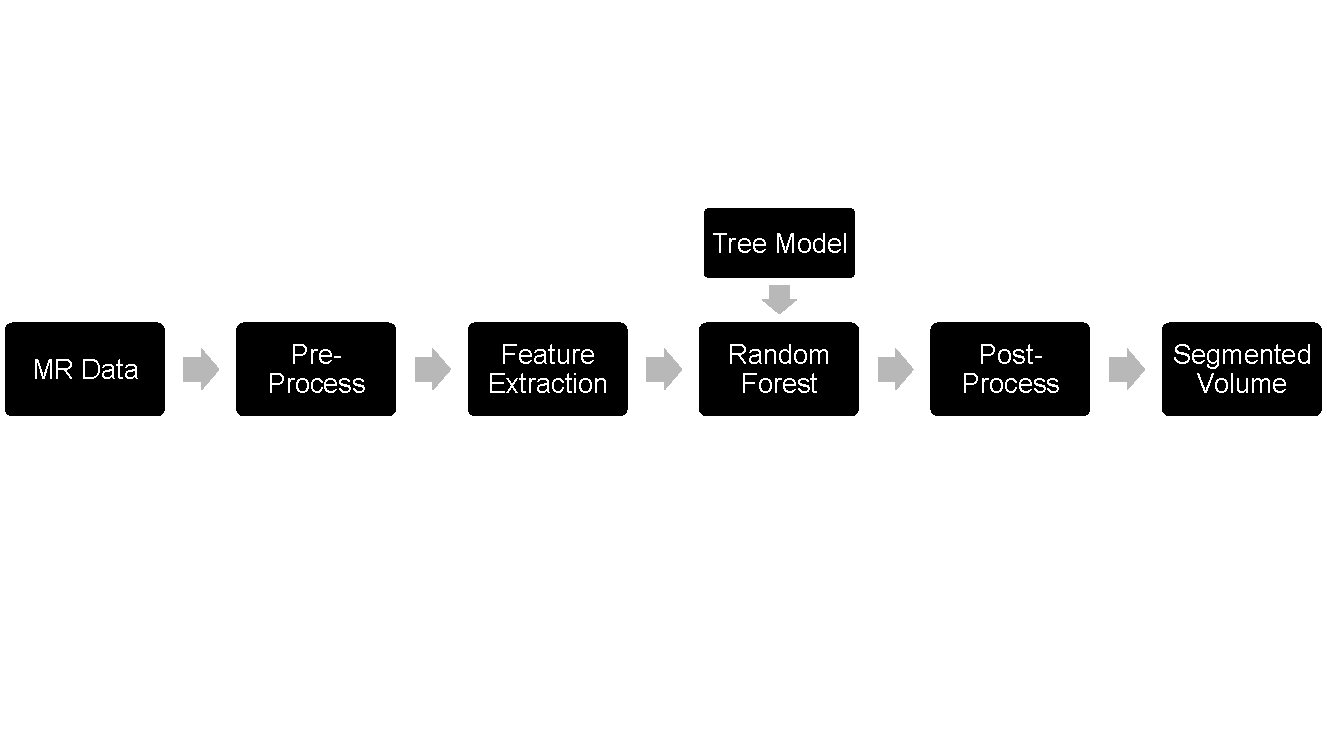
\includegraphics[width=\textwidth]{pipeline}
\caption{Pipeline of the proposed algorithm}
\label{fig:pipeline}
\end{figure*}

%fully automatic
%show the pipeline
%preprocessing (normlization, wiener filer), maybe show picture
%training, features, relative position, show kernels, number of trees, 2d features
%postprocessing, opening, largest area, filling, largest volume, show images as in presentation
%explain our cross validation procedure (DICE not OOB score)
